%% **************************** Sub Test ****************************
\setcounter{Sec}{0}\setcounter{Step}{0}

\newpage
\renewcommand{\subprocid}{{\procid}-02}

\newpage
\subsection{\subprocid \ Inrush and ripple measurement }


%% Test Setup
\begin{figure}[H]
	\centering
	  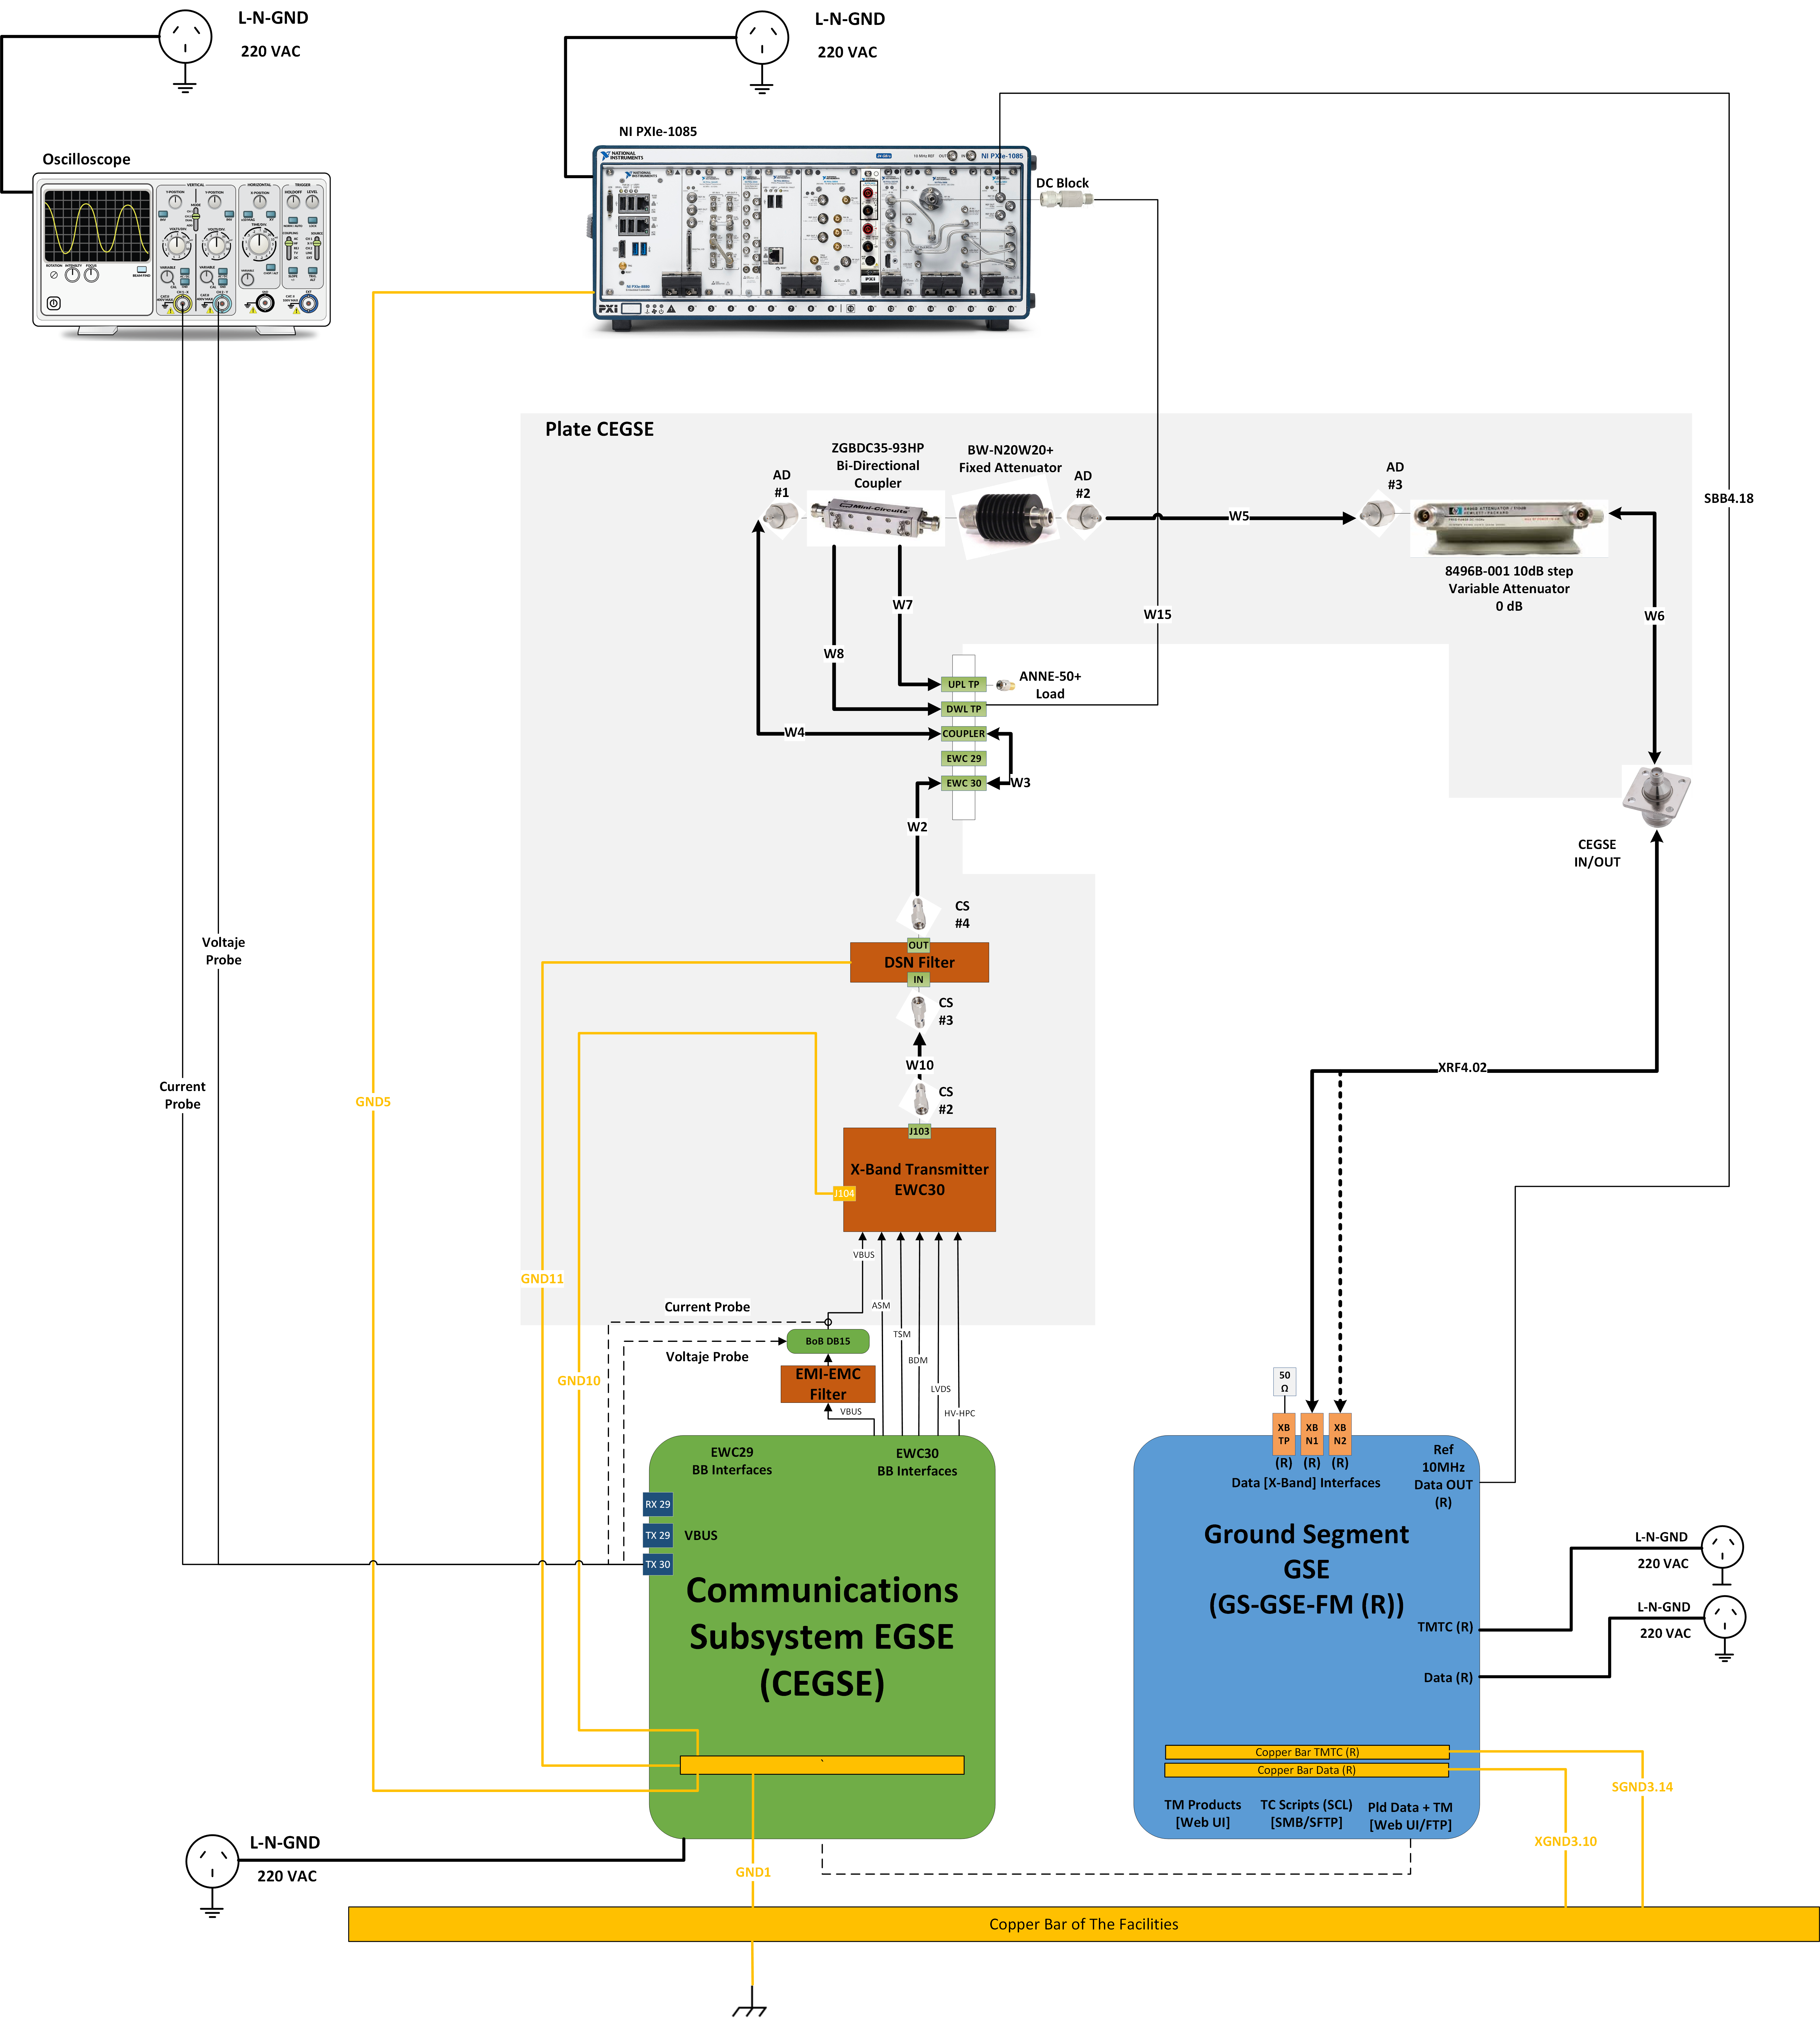
\includegraphics[width=.9\linewidth]{figuras/EWC30PXISetupA.png}  
	  \caption{EWC30 Inrush and ripple measurement setup.}
	\label{fig:setup_xband_funcional_ripple}
	\end{figure}
\newpage
\begin{stepstable}{\subprocid{} Inrush and ripple measurement.}
	\ExecutorRecord

	\SectionHeaderWithReset{Environmental temperature and humidity}
		\RegisterTempAndHumidity

	%%%%% Update %%%%%	
	\SectionHeaderWithReset{CEGSE power off (PXI and Ad-Hoc Box)}
		%\TurnOnOffVbusXBand{off}{}
		%\StopCegseSW{}
		\TurnOnOffPSU{off}
		\DisablePowerSupplyOutput
		\TurnOffMainSwitch
		\PowerOffPxi	
		%\ConfigDatalogger
	
	\SectionHeaderWithReset{DB-15 BOB connection to EMI/EMC filter}
		\DisconnectHarnessFromEMIEMCFilterOutput{\NuevoHarnessDos}
		\ConnectHarnessToEMIEMCFilterOutput{\NuevoHarnessCuatro} % Dos

		\ConnectTestHarnessToBreakOutBox{\NuevoHarnessCuatro}{DB-15 BOB}{female}
        
		% \ConnectHarnessToAdboxPowerSupplyOutput{\NuevoHarnessUno}
		% \ConnectHarnessToEMIEMCFilterInput{\NuevoHarnessUno}

		% \ConnectHarnessToEMIEMCFilterOutput{\NuevoHarnessDos} % Dos

		% \ConnectTestHarnessToDutHarness{\NuevoHarnessDos}{\NuevoHarnessTres}
		% \ConnectTestHarnessToBreakOutBox{\NuevoHarnessTres}{DB-15 BOB}{female}




	% \SectionHeaderWithReset{Preparation of GS-GSE}
	% 	\EnableNOneInterfaceXBand{Note: Skip this step if \textbf{EWC30-FM2} is under test.}
	% 	\EnableNTwoInterfaceXBand{Note: Skip this step if \textbf{EWC30-FM1} is under test.}
	% 	%\VerifyConfigurationInCortexHdr
	% 	\OpenWinCortexHDR

%%%%%%update %%
	\SectionHeaderWithReset{Power-on \comEgse{}}
		\TurnOnMainSwitch
		\VerifyPowerSupplyConfiguration{3 A}
		\EnablePowerSupplyOutput
		\TurnOnOffPSU{on}
		\PowerOnPxi
		\RDPToPXIFromThinClient{\thinDT A}

%%%%%%update %%
	\SectionHeaderWithReset{CEGSE SW Initialization}
		\StartCegseSW{EWC30}{"no alarm"}{"INIT\string_FILE\string_NO\string_ALARM\string_EWC30.ini"}
    
	\SectionHeaderWithReset{EWC30 Vbus verification}
		\TurnOnOffVbusXBand{on}{}
		\MeasureVBusOnBreakOutBox
		%\TurnOnOffVbusXBand{off}{}
		% \DisconnectTestHarnessToBreakOutBox{\NuevoHarnessTres}{female}
		% \DisconnectTestHarnessToDutHarness{\NuevoHarnessDos}{\NuevoHarnessTres}
		% \DisconnectHarnessFromEMIEMCFilterOutput{\NuevoHarnessDos}

		% \ConnectBOB{ DB-9}{J201B}
		% \ConnectBOB{DB-25}{J200 }
		% \ConnectBOB{DB-37}{J201A}
		
		%%%%%%update %%
	\SectionHeaderWithReset{CEGSE power off (PXI and Ad-Hoc Box)}
		\TurnOnOffVbusXBand{off}{}
		\StopCegseSW{}
		\TurnOnOffPSU{off}
		\DisablePowerSupplyOutput
		\TurnOffMainSwitch
		\PowerOffPxi	
		%\ConfigDatalogger

	\SectionHeaderWithReset{DB-15 BOB connection to DUT}
		
        \ConnectTestHarnessToBreakOutBox{\NuevoHarnessDos}{DB-15 BOB}{male}

		% \ConnectHarnessToAdboxPowerSupplyOutput{\NuevoHarnessUno}
		% \ConnectHarnessToEMIEMCFilterInput{\NuevoHarnessUno}

		% \ConnectHarnessToEMIEMCFilterOutput{\NuevoHarnessDos} % Dos

		% \ConnectTestHarnessToDutHarness{\NuevoHarnessDos}{\NuevoHarnessTres}
		% \ConnectTestHarnessToBreakOutBox{\NuevoHarnessTres}{DB-15 BOB}{female}
	%%%%%%%% Update %
	\SectionHeaderWithReset{Power-on \comEgse{}}
		\TurnOnMainSwitch
		\VerifyPowerSupplyConfiguration{3 A}
		\EnablePowerSupplyOutput
		\TurnOnOffPSU{on}
		\PowerOnPxi
		\RDPToPXIFromThinClient{\thinDT A}
	
	\SectionHeaderWithReset{PXI Spectrum Analyzer connection}
		\ConnectRfCableToDwlTpPortOfCegse{W15}{}
    	\ConnectCableToDcBlock{W15}

	\SectionHeaderWithReset{Instrument configuration}
		\StartPXISpectrumA
		\configPXISpectrumA{NI-RFSA-Data-N1.tdms if EWC30-FM1 is under test}{NI-RFSA-Data-N2.tdms if EWC30-FM2 is under test}
		\ConfigPowerBandPXI{195 MHz}
		\SectionHeaderWithReset{EGSE Settings}
		%\SetCegseVariableAttenuatorTo{1 dB}{5 dB}
		\SetCegseVariableAttenuatorTo{10 dB}{0 dB}
	\SectionHeaderWithReset{CEGSE SW Initialization}
		\StartCegseSW{EWC30}{Nominal}{INIT\string_FILE\string_EWC30.ini}{}

	\SectionHeaderWithReset{DUT Power On}
		\VerifyDutAlarms{EWC-30}{}
		\TakeNoteDutTemperaturesXBand{}
		\LoadOscilloscopeConfigFile{EWC30-TX-ON.set}{}
		\PressSingleOnOscilloscope
		\TurnOnOffVbusXBand{on}{}
		\TakeScreenShotOnOscilloscope
		\MeasureInrushCurrentOn{CH1}
		\SaveOscilloscopeRawValues
		\LoadOscilloscopeConfigFile{EWC30-TX-RUN.set}{}{}
		%\SimpleExeStep{\tr{validar cooriente y potencia}}{arg2}{arg3}
		\TakeNoteOfCurrentAndVoltageOf{TX}{CH1}{CH2}{28 V}{< 282 mA}{} 
		\VerifyPowerConsumptionOf{TX}{CH1}{CH2}{P $\approx$\ 8 W@standby}
		%\LoadOscilloscopeConfigFile{EWC30-TX-RIPPLE.set}{}
	
	
	\SectionHeaderWithReset{Verify DUT Telemetry}
		\VerifyRxSecondaryVoltageRFXBand
		\VerifyRxSecondaryVoltageNUMXBand
    	\VerifyRfOutputPowerTmXBand{< 0.5}
    	\VerifyTemperature{O\string_TX\string_TEMP1}{}
    	\VerifyClkLockedStatus{OFF}
    	\VerifyMmuClkStatus{OFF}
    	\VerifyTxStatusSBand{Standby}
		%\VerifyTxStatus{stand-by}{O\string_TX\string_STATUS = 0}

	% \SectionHeaderWithReset{Preparation of GS-GSE}
	% 	\EnableNOneInterfaceXBand{Note: Skip this step if \textbf{EWC30-FM2} is under test.}
	% 	\EnableNTwoInterfaceXBand{Note: Skip this step if \textbf{EWC30-FM1} is under test.}
	% 	%\VerifyConfigurationInCortexHdr
	% 	\OpenWinCortexHDR
		
		%%%%%%%%%%%%%%%%%%%%%%%%%%%%%%%%%%%%%%%%%%%%%%%%%%%%%%%%%%%%%%%%%%%%%%%%%%%%%%%%%%%%%%%%%%%%%%%%%%%%%%%%%%%
		% Medicioens de corriente  de ripple
		%%%%%%%%%%%%%%%%%%%%%%%%%%%%%%%%%%%%%%%%%%%%%%%%%%%%%%%%%%%%%%%%%%%%%%%%%%%%%%%%%%%%%%%%%%%%%%%%%%%%%%%%%%%
	\SectionHeaderWithReset{File generation for data transmission}
		\GenerateDownlinkFileXBand{1330000 ($\approx$180 seconds)}{1330000}{Data-885840\_120s\_VCh01\_payload.bin}{}
	\SectionHeaderWithReset{Ripple measurement between EMI/EMC filter and Ad-Hoc Box}
	\VerifyTemperature{O\string_TX\string_TEMP1}{}
		\SendGeneratedFileXBand{I\_STBY\_2\_OPE\_M}{main}
		\VerifyTxStatusXBand{Modulation}
		%\CheckLookCortexHDR
    	%\StartIngestionInCortexHdr
        %%%%%%%%Update %%
		\VerifyRxSecondaryVoltageRFXBand % mezcla
		\VerifyRxSecondaryVoltageNUMXBand % mezcla
		\VerifyRfOutputPowerTmXBand{$\approx$ 3.2}

		\VerifyClkLockedStatus{ON}
		\VerifyMmuClkStatus{ON} % de mezcla



	%	\VerifyClkLockedStatus{ON}
  		\TakeNoteOfCurrentAndVoltageOf{TX}{CH1}{CH2}{28\ V}{$\approx$ \ValueCurrentDUTTX A}{\notaCorrienteEstimada}
		\LoadOscilloscopeConfigFile{EWC30-TX-RIPPLE.set}{}
		\adquicicionOSCStop
		\TakeScreenShotOnOscilloscope
		\SaveOscilloscopeRawValues
		\adquicicionOSCStart
		\ChangeTimeConf
		\adquicicionOSCStop
		\TakeScreenShotOnOscilloscope
		\SaveOscilloscopeRawValues
		\TakeNoteOfCurrentAndVoltageRippleOf{TX}{CH1}{CH2}{\ValueVRipple}{\ValueIRippleADHBoxToFilter}
 %%% update
		\MeasureCarrierPowerModUsingPxi{40\ }{1} % de mezcla
		\TakeScreenShotOnPxi  % de mezcla
        %%%%%% Update %%%%%%%
		\ChangeTxStatusTo{I\string_OPE\string_2\string_STBY\string_M }{standby}
		\VerifyTxStatusXBand{Standby}
		%\StopXB
		\WaitUntilTxFinishedOnCegse

  %%%%%%%%%%% Update %%%%%%
    \SectionHeaderWithReset{DUT Turn Off}
		\LoadOscilloscopeConfigFile{EWC30-TX-OFF.set}{}
		\PressSingleOnOscilloscope
		\TurnOnOffVbusXBand{off}{}
		\TakeScreenShotOnOscilloscope
		\MeasurePowerDownCurrentOn{CH1}
		\SaveOscilloscopeRawValues
		\StopCegseSW{}

%%%%%%%%%%%% UPdate %%
	\SectionHeaderWithReset{Connections of oscilloscope probe between EMI/EMC filter and DUT}
		\ConnectMeasurementProbeBetweenFilterAndDUT
		\ConnectMeasurementVoltageProbeBetweenFilterAndDUT		
	%%%%% Update %%
	\SectionHeaderWithReset{CEGSE SW Initialization}
		\StartCegseSW{EWC30}{Nominal}{INIT\string_FILE\string_EWC30.ini}{}

%%%%%%%%%%%%%%% update %%%%
	\SectionHeaderWithReset{DUT Power On}
		\VerifyDutAlarms{EWC-30}{}



		%\TakeNoteDutTemperaturesXBand{}
		\VerifyTemperature{O\string_TX\string_TEMP1}{}

		 \LoadOscilloscopeConfigFile{EWC30-TX-ON.set}{}
		 \PressSingleOnOscilloscope
		 \TurnOnOffVbusXBand{on}{}
		 \TakeScreenShotOnOscilloscope
		 \MeasureInrushCurrentOn{CH1}
		 \SaveOscilloscopeRawValues
		\LoadOscilloscopeConfigFile{EWC30-TX-RUN.set}{}{}
		%\SimpleExeStep{\tr{validar cooriente y potencia}}{arg2}{arg3}
		\TakeNoteOfCurrentAndVoltageOf{TX}{CH1}{CH2}{28 V}{< 282 mA}{} 
		\VerifyPowerConsumptionOf{TX}{CH1}{CH2}{P $\approx$\ 8 W@standby}
		%\LoadOscilloscopeConfigFile{EWC30-TX-RIPPLE.set}{}
	
	%\SectionHeaderWithReset{File generation for data transmission}
	%	\GenerateDownlinkFileXBand{1330000 ($\approx$180 seconds)}{1330000}{Data-885840\_120s\_VCh01\_payload.bin}{}

    \SectionHeaderWithReset{Verify DUT Telemetry}
		\VerifyRxSecondaryVoltageRFXBand
		\VerifyRxSecondaryVoltageNUMXBand
    	\VerifyRfOutputPowerTmXBand{< 0.5}
    	\VerifyTemperature{O\string_TX\string_TEMP1}{}
    	\VerifyClkLockedStatus{OFF}
    	\VerifyMmuClkStatus{OFF}
    	\VerifyTxStatusSBand{Standby}
	
	\end{stepstable}
    \begin{stepstable}{\subprocid{} Inrush and ripple measurement.}
		
	\SectionHeaderWithReset{File generation for data transmission}
		\GenerateDownlinkFileXBand{1330000 ($\approx$180 seconds)}{1330000}{Data-885840\_120s\_VCh01\_payload.bin}{}

	\SectionHeaderWithReset{Ripple measurement between EMI/EMC filter and DUT}
		\VerifyTemperature{O\string_TX\string_TEMP1}{}
		\SendGeneratedFileXBand{I\_STBY\_2\_OPE\_M}{main}
		\VerifyTxStatusXBand{Modulation}
		%\CheckLookCortexHDR
    	%\StartIngestionInCortexHdr

		\VerifyRxSecondaryVoltageRFXBand % mezcla
		\VerifyRxSecondaryVoltageNUMXBand % mezcla
		\VerifyRfOutputPowerTmXBand{$\approx$ 3.2}

		\VerifyClkLockedStatus{ON}
		\VerifyMmuClkStatus{ON} % de mezcla


		%\VerifyClkLockedStatus{ON}
  		\TakeNoteOfCurrentAndVoltageOf{TX}{CH1}{CH2}{28\ V}{$\approx$ \ValueCurrentDUTTX A}{\notaCorrienteEstimada}



		\LoadOscilloscopeConfigFile{EWC30-TX-RIPPLE.set}{}
		\adquicicionOSCStop
		\TakeScreenShotOnOscilloscope
		\SaveOscilloscopeRawValues
		\adquicicionOSCStart
		\ChangeTimeConf
		\adquicicionOSCStop
		\TakeScreenShotOnOscilloscope
		\SaveOscilloscopeRawValues
		%\TakeNoteOfCurrent{TX}{CH1}{\ValueIRippleDUTToFilter}
		\TakeNoteOfCurrentAndVoltageRippleOf{TX}{CH1}{CH2}{\ValueVRipple}{\ValueIRippleADHBoxToFilter}

		\MeasureCarrierPowerModUsingPxi{40\ }{1} % de mezcla
		\TakeScreenShotOnPxi  % de mezcla

		%\adquicicionOSCStart
		%\ConnectMeasurementProbesToAdHocBoxForXBand
		%\LoadOscilloscopeConfigFile{EWC30-TX-RUN.set}{}{}
		%\WaitUntilTxFinishedOnCegse
		%\StopIngestonInCortexHdr
		\ChangeTxStatusTo{I\string_OPE\string_2\string_STBY\string_M }{standby}
		\VerifyTxStatusXBand{Standby}
		%\StopXB
		\WaitUntilTxFinishedOnCegse
			%%%%%%%%%%% Update %%%%%%
	\SectionHeaderWithReset{DUT Turn Off}
		\LoadOscilloscopeConfigFile{EWC30-TX-OFF.set}{}
		\PressSingleOnOscilloscope
		\TurnOnOffVbusXBand{off}{}
		\TakeScreenShotOnOscilloscope
		\MeasurePowerDownCurrentOn{CH1}
		\SaveOscilloscopeRawValues
		%\StopCegseSW{}
	%%%%%%%%%%%%%%%%%%%%%%%%%%%%%%%%%%%%%%%%%%%%%%%%%%%%%%%%%%%%%%%%%%%%%%%%%%%%%%%%%%%%%%%%%%%%%%%%%%%%%%%%%%%
    %%%%%%%%%%%%%%%%%%%%%%%%%%%%%%%%%%%%%%%%%%%%%%%%%%%%%%%%%%%%%%%%%%%%%%%%%%%%%%%%%%%%%%%%%%%%%%%%%%%%%%%%%%%

%    \SectionHeaderWithReset{File generation for data transmission}
%      \GenerateDownlinkFileXBand{1000000 ($\approx$135 seconds)}{1000000}{Data-885840\_120s\_VCh01\_payload.bin}{}

% 	\SectionHeaderWithReset{RF measurements with the PXI Spectrum Analyzer and Data Downlink test}
%    		\VerifyTemperature{O\string_TX\string_TEMP1}{}
% 		\SendGeneratedFileXBand{I\_STBY\_2\_OPE\_R}{redundant}
% 		\VerifyTxStatusXBand{Modulation}
% 		\CheckLookCortexHDR
%     	\StartIngestionInCortexHdr
% 		\VerifyRxSecondaryVoltageRFXBand % mezcla
% 		\VerifyRxSecondaryVoltageNUMXBand % mezcla
% 		\VerifyClkLockedStatus{ON}
% 		\VerifyMmuClkStatus{ON} % de mezcla
% 		%\VerifyRfOutputPowerTmXBand{$\approx$ 3.2} % estaba antes
% 		%\LoadOscilloscopeConfigFile{EWC30-TX-RIPPLE.set}{}{}
% 		%\adquicicionOSCStop
% 		%\TakeScreenShotOnOscilloscope
% 		%\SaveOscilloscopeRawValues
% 		%\adquicicionOSCStart
% 		%\ChangeTimeConf
% 		%\adquicicionOSCStop
% 		%\TakeScreenShotOnOscilloscope
% 		%\SaveOscilloscopeRawValues
% 		%\TakeNoteOfCurrentAndVoltageRippleOf{TX}{CH1}{CH2}{542\ mVpp}{750\ mApp}
% 		%\adquicicionOSCStart
        
% 		\VerifyRfOutputPowerTmXBand{$\approx$ 3.2} % de mezcla
% 		\TakeNoteOfCurrentAndVoltageOf{TX}{CH1}{CH2}{28\ V}{$\approx$ \ValueCurrentDUTTX A}{\notaCorrienteEstimada}
% 		\MeasureCarrierPowerModUsingPxi{40\ }{1} % de mezcla
% 		\TakeScreenShotOnPxi  % de mezcla
% 		\ConfigBandWidthPXI   % de mezcla
% 		\MeasureOccupiedBandwidthUsingPxi{205} % de mezcla
% 		\TakeScreenShotOnPxi  % de mezcla



% 		\WaitUntilTxFinishedOnCegse
% 		\StopIngestonInCortexHdr
% 		\MeasureLOLeakageUsingPxi % de mezcla
% 		\ChangeTxStatusTo{I\string_OPE\string_2\string_STBY\string_R }{standby} % de mezcla
% 		%\ChangeTxStatusTo{I\string_OPE\string_2\string_STBY\string_M }{standby}
% 		\VerifyTxStatusXBand{Standby} % de mezcla
% 		%\VerifyTxStatusXBand{Standby}

% 	\SectionHeaderWithReset{Verify received data}
% 		\VerifyNumberOfIdlesFramesReceivedInCortexHdr
% 		\VerifyNumberOfFramesReceivedVCOneInCortexHdr{1}{885840}
% 		\StartDataRFFlow{1800}
% 		\WaitForDataFlowExecution
% 		\LoginToCCM
% 		\GoToProductsOnCCM
% 		\FindXBandProductOnCCM
% 		\DownloadIdentifiedProductFromCCM{}
% 		\RemoveTransportLayer{X Band}{885840}
% 		\CompareDownlinkPayloadFiles{EWC30}{\fileXbCompare}
		
%     \SectionHeaderWithReset{RF measurements with the PXI Spectrum Analyzer}
% 		\VerifyTemperature{O\string_TX\string_TEMP1}{}
% 		\SendGeneratedFileXBand{I\_STBY\_2\_OPE\_R}{redundant}
% 		\VerifyTxStatusXBand{Modulation}
% 		\CheckLookCortexHDR
% 		\VerifyRxSecondaryVoltageRFXBand
% 		\VerifyRxSecondaryVoltageNUMXBand
% 		\VerifyClkLockedStatus{ON}
% 		\VerifyMmuClkStatus{ON}
% 		\VerifyRfOutputPowerTmXBand{$\approx$ 3.2}
% 		\MeasureCarrierPowerModUsingPxi{40\ }{1}
% 		\TakeScreenShotOnPxi 
% 		\ConfigBandWidthPXI
% 		\MeasureOccupiedBandwidthUsingPxi{205}
% 		\TakeScreenShotOnPxi 
% 		\WaitUntilTxFinishedOnCegse
% 		\MeasureLOLeakageUsingPxi
% 		\ChangeTxStatusTo{I\string_OPE\string_2\string_STBY\string_R }{standby}
% 		\VerifyTxStatusXBand{Standby}

	% \SectionHeaderWithReset{DUT Turn Off}
	% 	%\LoadOscilloscopeConfigFile{EWC30-TX-OFF.set}{}
	% 	%\PressSingleOnOscilloscope
	% 	\TurnOnOffVbusXBand{off}{}
	% 	%\TakeScreenShotOnOscilloscope
	% 	%\MeasurePowerDownCurrentOn{CH1}
	% 	%\SaveOscilloscopeRawValues
	
	% \SectionHeaderWithReset{CEGSE SW Shutdown}
	% 	\StopCegseSW{}

    
    	%%%%%%update %%
	\SectionHeaderWithReset{CEGSE power off (PXI and Ad-Hoc Box)}
	%\TurnOnOffVbusXBand{off}{}
	\StopCegseSW{}
	\TurnOnOffPSU{off}
	\DisablePowerSupplyOutput
	\TurnOffMainSwitch
	\PowerOffPxi	
	%\ConfigDatalogger
	\SectionHeaderWithReset{DB-15 BOB disconnection and DUT connection}
	 \DisconnectTestHarnessToBreakOutBox{\NuevoHarnessDos}{male}
	 \DisconnectTestHarnessToBreakOutBox{\NuevoHarnessCuatro}{female}
	 \DisconnectHarnessFromEMIEMCFilterOutput{\NuevoHarnessCuatro}
	 \ConnectHarnessToEMIEMCFilterOutput{\NuevoHarnessDos} % Dos

    
		%\ConnectTestHarnessToBreakOutBox{\NuevoHarnessCuatro}{DB-15 BOB}{female}
        
		% \ConnectHarnessToAdboxPowerSupplyOutput{\NuevoHarnessUno}
		% \ConnectHarnessToEMIEMCFilterInput{\NuevoHarnessUno}

		% \ConnectHarnessToEMIEMCFilterOutput{\NuevoHarnessDos} % Dos

		% \ConnectTestHarnessToDutHarness{\NuevoHarnessDos}{\NuevoHarnessTres}
		% \ConnectTestHarnessToBreakOutBox{\NuevoHarnessTres}{DB-15 BOB}{female}

	%%%%%%update %%
	\SectionHeaderWithReset{Power-on \comEgse{}}
		\TurnOnMainSwitch
		\VerifyPowerSupplyConfiguration{3 A}
		\EnablePowerSupplyOutput
		\TurnOnOffPSU{on}
		\PowerOnPxi
		\RDPToPXIFromThinClient{\thinDT A}
	

	\SectionHeaderWithReset{Collect Evidences}
		\CopyCegseLogsForEvicences{\subprocid}{}
		\CopyOscilloscopeScreenShotsForEvidences
		\GetTempAndHumidityFromDatalogger
		%\ConnectPendriveTo{oscilloscope}

	\SectionHeaderWithReset{Final Steps}
		%\SetReduntanSideOnXbmaDisableMandC
		\RegisterTempAndHumidity
		\DisconnectRfCableFromDwlTpOfCegse{W15}{\pasarSiDespues}
		\DisconnectCableFromDcBlock{W15}{\pasarSiDespues} 
		\ClosePXISA
		\ConnectMeasurementProbesToAdHocBoxForXBand	
		\ConnectPendriveTo{Oscilloscope}
	

		%\ClosePXIM 

\end{stepstable}
\begin{longtable}{|p{17.0cm}|}
	\endfirsthead
	\endfoot
	\caption{Procedure \subprocid \ table.} \label{tb:proc:018-02}
\end{longtable}
